\documentclass[
  % fourier,
  % print,
]{tudelft-report}[2026/06/01]

% UK English is the default language; Dutch for designated parts
\ifluatex
  \RequirePackage{polyglossia}
  \setdefaultlanguage[variant=british]{english}
  \setotherlanguage{dutch}
  % define babel syntax when using polyglossia, so we can use either package
\else
  % american is needed for \blindtext and \blinddocument
  \RequirePackage[dutch,american,british]{babel}
  % \NewDocumentEnvironment{dutch}{\begin{foreignlanguage}{dutch}}{\end{foreignlanguage}}
\fi
\RequirePackage{csquotes}

\usepackage[
  % style=apa,
]{biblatex}
\addbibresource{report.bib}

\usepackage{changes}
\usepackage[math]{blindtext} % filler text

\usepackage{enumitem} % for a., b., c. and i., ii., iii. sub-lists in the assignment questions
\usepackage{booktabs} % for the torsion/warping constants table in Assignment 5
\usepackage{verbatim} % \verbatiminput of the calculation scripts in the appendix

% Hyperlinks are blue, except in print mode, when they are all black.
\usepackage[
  colorlinks=true,
  citecolor=accent,
  linkcolor=accent,
  urlcolor=accent,
]{hyperref}


\begin{document}

% metadata such as author, title, etc. are defined in cover.tex
% arara: pdflatex
% we will use commands containing `@' in the name:
\makeatletter
\newif\if@onlycoverfront
\ifx\@onlypreamble\@notprerr
  % latex already read a \begin{document}
  % so now our job is to output just the of the front cover
  % as part of the full report
  \@onlycoverfronttrue
\else
  % latex did not read a \begin{document}
  % so now our job is to output the full cover
  \@onlycoverfrontfalse
  \documentclass{tudelft-report}[2026/06/01]
  \begin{document}
\fi

% this file can either be compiled on its own, or as part of the main document
% as part of the main document, it is only supposed to create a front cover
% and (re)define a command \MakeCoverBack to add the back cover to the document.

% document metadata
\title{Advanced Mechanics of Maritime Structures}
\subtitle{MT44030 -- Assignment Report}
\author{Student Name \& Student Name}
\newcommand{\isbn}{MT44030}

% set lengths used for the cover
\setcoverbleed{1.5mm}
\newlength{\covermargin}
\setlength{\covermargin}{30mm}

\let\oldoddsidemargin\oddsidemargin
\usetikzlibrary{fadings,patterns}

% everything is pretty free format, since it would probably be impossible to
% create a cover template that will make everyone happy


\begin{tikzfadingfrompicture}[name=myfading radial]
\draw[inner color=transparent!40, outer color=transparent!100] (0,0) rectangle (2,2);
\end{tikzfadingfrompicture}

\renewcommand{\CoverFront}{%
  \begin{tikzpicture}[overlay, inner sep=0pt]
    \node[anchor=south west] at (-\coverspinewidth, -\coverbleed)
      {\pgfimage[width=\dimexpr(\oldpaperwidth+\coverspinewidth+2\coverbleed)\relax]{tank-below.jpg}};
    \node[anchor=north west]% define upper left corner
      at (30mm, \oldpaperheight-30mm)
      {{\begin{minipage}%
          [t]% vertical alignment of minipage w.r.t. surroundings; irrelevant since it is in a tikz node here
          [90mm]% height of minipage
          [b]% vertical alignment of text within minipage
          {\dimexpr(\oldpaperwidth-60mm)\relax}% width of minipage
        \KOMAoptions{parskip=half}
        \raggedright
        \color{white}
        % hard-coded formatting, since it's hard to predict what is sensible
        {\headingfont
          {\fontsize{60pt}{60pt}\selectfont\@title\\[20pt]}
          \ifx\@subtitle\@empty\else
            {\fontsize{30pt}{30pt}\selectfont\@subtitle\\[30pt]}
          \fi
        }
        \color{black}
        {\makeatletter\Huge\@author\makeatother}
        \vfill
        \large
        \textbf{Faculty of Mechanical Engineering}\\[1ex]
        Department of Maritime and Transport Technology

        \isbn
      \end{minipage}}
    };
    % darken background slightly so logo is more visible
    \fill[black, path fading=myfading radial] (0cm,0cm) rectangle (17cm,7cm);
    \node[anchor=south west, scale=4] at (\covermargin, \covermargin) {\tudlogo[white]};    
  \end{tikzpicture}
}

% has to be inserted manually in the main document
\renewcommand{\CoverBack}{%
  \tikz[overlay]{
    \node[
      anchor=south west,
      scale=4,
    ] at (\covermargin, \covermargin)
    {\tudlogo[white]};
  }
}

\MakeCoverFront%

\if@onlycoverfront
  \endinput
\fi

% define what has to be printed on the spine, which will be placed between the
% front and back cover in the output of \MakeCoverFull
\renewcommand{\CoverSpine}{%
  \tikz[overlay]{%
    \node[
      anchor=west,
      rotate=90,
      minimum height=\coverspinewidth,
      fill=black,
      text=white,
    ]
    at (0.5\coverspinewidth, 0.7\paperheight)
    {\quad\@title \hspace*{\paperheight}};
  }
}

\MakeCoverFull%

\renewcommand{\CoverFront}{%
  \begin{tikzpicture}[overlay, inner sep=0pt]
    % background image
    \node[anchor=south west] (bg) at (-\coverspinewidth, -2cm)
      {\pgfimage[width=\dimexpr(\oldpaperwidth+\coverspinewidth+2\coverbleed)\relax]{tank-overview.jpg}};
    % darken the top so that the text is more visible
    \tikzfading[name=fade down, top color=transparent!50, bottom color=transparent!100]
    \fill[black, path fading=fade down] (bg.north west) rectangle (bg.east);
    % text area
    \node[anchor=south west]% define lower left corner
      at (30mm, 20mm)
      {{\begin{minipage}%
          [t]% vertical alignment of minipage w.r.t. surroundings; irrelevant since it is in a tikz node here
          [\dimexpr(\oldpaperheight-50mm)\relax]% height of minipage
          [b]% vertical alignment of text within minipage
          {\dimexpr(\oldpaperwidth-60mm)\relax}% width of minipage
        \KOMAoptions{parskip=half}
        \raggedright
        \color{white}
        % free format / hard-coded formatting, since it's hard to predict what is sensible
        {\headingfont
          {\fontsize{60pt}{60pt}\selectfont\@title\\[20pt]}
          \ifx\@subtitle\@empty\else
            {\fontsize{30pt}{30pt}\selectfont\@subtitle\\[30pt]}
          \fi
        }
        {\makeatletter\Huge\@author\makeatother}
        \vfill
        \large
        \textbf{Faculty of Mechanical Engineering}\\[1ex]
        Department of Maritime and Transport Technology

        \isbn
        
        \bigskip

        % logo with asterisk hides "Delft University of Technology", which would not look nice on this specific background
        \scalebox{3}{\tudlogo*[white]}
        \end{minipage}}
    };
  \end{tikzpicture}
}

\makeatother

\MakeCoverFront%

\MakeCoverFull%

\MakeCoverBack%

\end{document}


% Use Roman numerals for the page numbers of the title pages and table of
% contents.
\frontmatter

% Include an optional title page.
\begin{titlepage}

\begin{center}

% Print the title in large font
{\makeatletter\headingfont
\fontsize{60}{60}\selectfont\@title{}
\makeatother}

% Print the optional subtitle
{\makeatletter
\ifx\@subtitle\undefined\else
  \bigskip
  {\headingfont\fontsize{22}{32}\selectfont\@subtitle}
\fi
\makeatother}

\bigskip
\bigskip

\iflanguage{dutch}{door}{by}

\bigskip
\bigskip

% Print the name of the author
{\makeatletter
\fontsize{26}{26}\selectfont\@author{}
\makeatother}

\bigskip
\bigskip

\iflanguage{dutch}{
  ter verkrijging van de graad van Master of Science

  aan de TU Delft,

  in het openbaar de verdedigen op dinsdag 1 januari om 10:00 uur.
}{
  to obtain the degree of Master of Science

  at the TU Delft,

  to be defended publicly on Tuesday January 1, 2013 at 10:00 AM.
}

\vfill

\begin{tabular}{lll}
  Student number: & 1234567 \\
  Project duration: & \multicolumn{2}{l}{March 1, 2012 -- January 1, 2013} \\
  Thesis committee: & Prof.\ dr.\ ir.\ J.\ Doe, & TU Delft, supervisor \\
    & Dr.\ E.\ L.\ Brown, & TU Delft \\
    & Ir.\ A.\ Aaronson, & Acme Corporation
\end{tabular}

\bigskip
\bigskip
% Only include the following lines if confidentiality is applicable.
\emph{\iflanguage{dutch}%
  {Op dit verslag is geheimhouding van toepassing tot en met 31 december 2013.}%
  {This thesis is confidential and cannot be made public until December 31, 2013.}%
}

\bigskip
\bigskip
An electronic version of this thesis is available at \url{http://repository.tudelft.nl/}.

% Insert the TU Delft logo at the bottom of the page.
\vspace{25mm}
\makeatletter
\scalebox{3}{
  \if@print%
    \tudlogo[black]
  \else
    \tudlogo%
  \fi
}
\makeatother
\end{center}

\end{titlepage}


\chapter{Preface}

This report has been prepared for the course \textbf{MT44030 -- Advanced Mechanics of Maritime Structures} at Delft University of Technology (2026 edition).

The chapter structure of this report mirrors the assignment brief one-to-one: \textbf{Part~1} (Chapters~\ref{ch:assignment1}--\ref{ch:assignment3}) covers Assignments~1--3, and \textbf{Part~2} (Chapters~\ref{ch:assignment4}--\ref{ch:assignment7}) covers Assignments~4--7. Within each chapter, section numbers match the question numbers of the corresponding assignment (e.g.\ \S3.4 answers Question~3.4).

\bigskip
\noindent\textbf{Group members:}
\begin{itemize}
  \item Aymen el Moubarik (5597617)
  \item Name (student number)
\end{itemize}

\begin{flushright}
{\makeatletter\itshape
  \@author\\
  Delft, \today
\makeatother}%
\end{flushright}


\tableofcontents

% Use Arabic numerals for the page numbers of the chapters.
\mainmatter%

\chapter{Introduction}

This document is intended to be both an example of the TU Delft \LaTeX{} template for reports which can be used for both BSc and MSc theses, as well as a short introduction to its use. It is not intended to be a general introduction to \LaTeX{} itself,\footnote{We recommend \url{http://en.wikibooks.org/wiki/LaTeX} as a reference and a starting point for new users.} and we will assume the reader to be familiar with the basics of creating and compiling documents.

Instructions on how to use this template under Windows, Linux and MacOS, and which \LaTeX{} packages are required, can be found in \texttt{README.txt}.


\section{Document Structure}

Since a report, and especially a thesis, might be a substantial document, it is convenient to break it up into smaller pieces. In this template we therefore give every chapter its own file. The chapters (and appendices) are gathered together in \texttt{report.tex}, which is the master file describing the overall structure of the document. \texttt{report.tex} starts with the line
\begin{verbatim}
  \documentclass{tudelft-report}
\end{verbatim}
which loads the TU Delft report template. The template is based on the \LaTeX{} \texttt{scrbook} document class and stored in \texttt{tudelft-report.cls}. The document class accepts several comma-separated options. The default language is (UK) English, but this can be changed to Dutch (\emph{e.g.}, for bachelor theses) by specifying the \texttt{dutch} option:
\begin{verbatim}
  \documentclass[dutch]{tudelft-report}
\end{verbatim}
Furthermore, hyperlinks are shown in blue, which is convenient when reader the report on a computer, but can be expensive when printing and does not serve the purpose it has in a digital document. They can be turned black with the \texttt{print} option. This will also turn the chapter numbers grey instead of light blue.

If the document becomes large, it is easy to miss warnings about the layout in the \LaTeX{} output. In order to locate problem areas, add the \texttt{draft} option to the \texttt{\textbackslash documentclass} line. This will display a vertical bar in the margins next to the paragraphs that require attention.

This template has the option to generate a cover page by including the file \texttt{cover.tex}. See the next section for a detailed description.

The contents of the report are included between the \texttt{\textbackslash{}begin\{document\}} and \texttt{\textbackslash{}end\{docu\-ment\}} commands, and split into four parts by
\begin{enumerate}
  \item \texttt{\textbackslash{}frontmatter}, which uses Roman numerals for the page numbers and is used for the title page and the table of contents;
  \item \texttt{\textbackslash{}mainmatter}, which uses Arabic numerals for the page numbers and is the style for the chapters;
  \item \texttt{\textbackslash{}appendix}, which uses letters for the chapter numbers, starting with `A'.
  \item \texttt{\textbackslash{}backmatter}, which has no chapter numbers at all.
\end{enumerate}
The title page is defined in a separate file, \texttt{title.tex}. Additionally, it is possible to include a preface, containing, for example, the acknowledgements. An example can be found in \texttt{preface.tex}. The table of contents is generated automatically with the \texttt{\textbackslash{}tableofcontents} command. Chapters are included after \texttt{\textbackslash{}mainmatter} and appendices after \texttt{\textbackslash{}appendix}. For example, \texttt{\textbackslash include\{in\-troduction\}} includes \texttt{introduction.tex}.

\subsection{Bibliography}

Lists of references are handled by \texttt{biblatex}.
The present document has the following preamble
\begin{verbatim}
\usepackage[style=apa]{biblatex}
\addbibresource{report.bib}
\end{verbatim}
The first line tells us that the references will be formatted according 
to the APA-standards.

The second line points to a file that contains the references in a database-like format.
Use one such line for every database that you want to use.

The general way this works is as follows (using the present document as an example):
\begin{verbatim}
lualatex report
biber report
lualatex report
lualatex report
\end{verbatim}
The first line typesets the document and gathers information for the lists of references; the second line will generate lists of references for all chapters, these will be read in during execution of the third and fourth lines.
The repetition of \texttt{lualatex report} is needed to get all the page numbers in links and references right.
Depending on the editor that you use much of this can be done by clicking on a suitable icon or by hitting suitably defined hot keys. On Overleaf, all of this is done when you press \texttt{ctrl+r} or \texttt{ctrl+enter}.

The \texttt{biblatex} package has many options and can be tailored to almost every need; you can explore its documentation at \texttt{https://www.ctan.org/pkg/biblatex}

To get numbered references just use
\begin{verbatim}
\usepackage{biblatex}
\addbibresource{report.bib}
\end{verbatim}
That is, remove \texttt{style=apa}.

To give some examples we cite an article: \textcite{Einstein1906},
a book: \textcite{MR1039321}, another article: \textcite{MR3860876},
and a book with more than one editor: \textcite{MR3204729}.


\section{Cover and Title Page}

This template will automatically generate a cover page if you include the file \texttt{cover.tex}.
This file defines three commands:

\texttt{\textbackslash{}MakeCoverFront} inserts just the front cover

\texttt{\textbackslash{}MakeCoverFull} inserts the complete cover (front, back, and spine) with some `bleed', i.e., a slightly enlarged edge to allow for cutting of the page after printing.

\texttt{\textbackslash{}MakeCoverBack} inserts just the back cover

\texttt{cover.tex} can be adapted according to your liking; this process is relatively free-format, with some examples given in \texttt{cover.tex}.

For a thesis it is desirable to have a title page within the document, containing information like the thesis committee members. To give you greater flexibility over the layout of this page, it is described in the file \texttt{title.tex}. Modify this file according to your needs. The example text is in English, but Dutch translations are provided in the comments. Note that for a thesis, the title page is subject to requirements which differ by faculty. Make sure to check these requirements before printing.


\section{Chapters}

Each chapter has its own file. For example, the \LaTeX{} source of this chapter can be found in \texttt{introduc\-tion.tex}. A chapter starts with the command
\begin{verbatim}
  \chapter{Chapter title}
\end{verbatim}
This starts a new page, prints the chapter number and title and adds a link in the table of contents. If the title is very long, it may be desirable to use a shorter version in the page headers and the table of contents. This can be achieved by specifying the short title in brackets:
\begin{verbatim}
  \chapter[Short title]{Very long title with many words 
    which could not possibly fit on one line}
\end{verbatim}

Chapters are subdivided into sections, subsections, subsubsections, and, optionally, paragraphs and subparagraphs. All can have a title, but only sections and subsections are numbered:
\section{\textbackslash section\{\ldots\}}
\subsection{\textbackslash subsection\{\ldots\}}
\subsubsection{\textbackslash subsubsection\{\ldots\}}
\paragraph{\textbackslash paragraph\{\ldots\}}

\section{Fonts and Colors}

The main font in this template is Arial, with the main headers in Roboto Slab, according to the TU Delft corporate style.
Alternatively, using the class option \texttt{\textbackslash{}documentclass[fourier]}, the serif font Utopia can be used (provided by the package \texttt{fourier}).
In that latter case, Helvetica will be used in the main headers.

The corporate colors of the TU Delft are \textcolor{tud Blue}{\textbf{blue}}, \textbf{black} and \textbf{white}, available, respectively, via \texttt{\textbackslash text\-color\{tud Blue\}\{...\}}, \texttt{\textbackslash textcolor\{black\}\linebreak[0]\{...\}} and \texttt{\textbackslash textcolor\{white\}\linebreak[0]\{...\}}.
Apart from these three, the house style defines the following basic colors, that can be used via \texttt{\textbackslash text\-color\{tud \textit{colorname}\}\{...\}}, where \texttt{\textit{colorname}} is any of:

\vspace{\topsep}\noindent
\begin{minipage}{.32\textwidth}
  \begin{itemize}
    \itemsep 0pt
    \parskip 0pt
    \item \textcolor{tud DarkBlue}{\textbf{Dark blue}}
    \item \textcolor{tud Turquoise}{\textbf{Turquoise}}
    \item \textcolor{tud RoyalBlue}{\textbf{Royal blue}}
    \item \textcolor{tud LightPurple}{\textbf{Light purple}}
  \end{itemize}
\end{minipage}
\begin{minipage}{.32\textwidth}
  \begin{itemize}
    \itemsep 0pt
    \parskip 0pt
    \item \textcolor{tud Pink}{\textbf{Pink}}
    \item \textcolor{tud Burgundy}{\textbf{Burgundy}}
    \item \textcolor{tud Red}{\textbf{Red}}
    \item \textcolor{tud Orange}{\textbf{Orange}}
  \end{itemize}
\end{minipage}
\begin{minipage}{.32\textwidth}
  \begin{itemize}
    \itemsep 0pt
    \parskip 0pt
    \item \textcolor{tud Yellow}{\textbf{Yellow}}
    \item \textcolor{tud Green}{\textbf{Green}}
    \item \textcolor{tud ForestGreen}{\textbf{Forest green}}
    \item \textcolor{tud DarkGrey}{\textbf{Dark grey}}
  \end{itemize}
\end{minipage}
\vspace{\topsep}

For shading of areas, specific reduced coverages of blue and dark grey may be used, but mind contrast and readability.
These reduced coverages are:
\begin{itemize} 
    \itemsep 0pt
    \parskip 0pt
  \item \textcolor{tud Blue}{\textbf{Blue:}}
    \tikz[baseline]{\node[fill=tud Blue!50, anchor=base] {50\,\%,};}%
    \tikz[baseline]{\node[fill=tud Blue!10, anchor=base] {10\,\%};}
  \item \textcolor{tud DarkGrey}{\textbf{Dark grey:}}
    \tikz[baseline]{\node[fill=tud DarkGrey!60, anchor=base] {\textcolor{white}{60\,\%,}};}%
    \tikz[baseline]{\node[fill=tud DarkGrey!40, anchor=base] {40\,\%,};}%
    \tikz[baseline]{\node[fill=tud DarkGrey!15, anchor=base] {15\,\%};}
\end{itemize}

Furthermore, there are paler versions of these colors to be used for data visualisation only:

\vspace{\topsep}\noindent
\begin{minipage}{.32\textwidth}
  \begin{itemize}
    \itemsep 0pt
    \parskip 0pt
    \item \textcolor{tud DarkBluePale}{\textbf{Dark blue}}
    \item \textcolor{tud TurquoisePale}{\textbf{Turquoise}}
    \item \textcolor{tud RoyalBluePale}{\textbf{Royal blue}}
    \item \textcolor{tud LightPurplePale}{\textbf{Light purple}}
  \end{itemize}
\end{minipage}
\begin{minipage}{.32\textwidth}
  \begin{itemize}
    \itemsep 0pt
    \parskip 0pt
    \item \textcolor{tud PinkPale}{\textbf{Pink}}
    \item \textcolor{tud BurgundyPale}{\textbf{Burgundy}}
    \item \textcolor{tud RedPale}{\textbf{Red}}
    \item \textcolor{tud OrangePale}{\textbf{Orange}}
  \end{itemize}
\end{minipage}
\begin{minipage}{.32\textwidth}
  \begin{itemize}
    \itemsep 0pt
    \parskip 0pt
    \item \textcolor{tud YellowPale}{\textbf{Yellow}}
    \item \textcolor{tud GreenPale}{\textbf{Green}}
    \item \textcolor{tud ForestGreenPale}{\textbf{Forest green}}
    \item \textcolor{tud DarkGreyPale}{\textbf{Dark grey}}
  \end{itemize}
\end{minipage}


\part{Part 1}
\chapter{Closed Section A}
\label{ch:assignment1}

\begingroup\itshape Assignment 1 --- 9 points\endgroup

\bigskip
This part of the assignment focuses on the aft of the vessel where the engine room is located (Section~A). In quartering waves, the vessel is subject to a torsional load. The shape of this closed section is approximated by a hollow triangle (see Figure~3 of the assignment brief), whose interior boundary is a scaled copy of the exterior boundary with scaling factor~$k$. To approximate the shear stresses resulting from a torsional moment applied to the section, the Prandtl stress function may be used; its contour is shown in Figure~4 of the assignment brief.

\section{Location of maximum shear stress}

Based on the displayed stress function, identify the location(s) of maximum shear stress $\tau_{xy}$ and $\tau_{xz}$. Include your reasoning. \textbf{(3 pts)}

\bigskip
\textit{Answer.}

\section{Inaccuracies of the Prandtl-based prediction}

Considering the mismatch between the inner boundary and the innermost contour lines, which inaccuracies are present in the Prandtl-based shear stress prediction? Mark the regions with the highest inaccuracy on the figure. \textbf{(3 pts)}

\bigskip
\textit{Answer.}

\section{Cross-sectional efficiency}

Consider that the outer boundary defines a solid cross section with area $A_{solid}$ and torsional constant $I_{p,solid}$.

Using $k$, express the areas $A_{inner}$ and $A_{hollow}$ in terms of $A_{solid}$, and the torsional constants $I_{p,inner}$ and $I_{p,hollow}$ in terms of $I_{p,solid}$. Obtain and plot the cross-sectional efficiency
\[
  \eta(k) = \frac{I_{p,hollow}/A_{hollow}}{I_{p,solid}/A_{solid}}.
\]
Discuss the balance between the cross-sectional efficiency and strength. \textbf{(3 pts)}

\bigskip
\textit{Answer.}

\chapter{Open Sections B}
\label{ch:assignment2}

\begingroup\itshape Assignment 2 --- 20 points\endgroup

\bigskip
For section~B two configurations are at hand (designs B1 and B2). This section is the parallel midship of the vessel and has tanks in the side shells and a double bottom. $M_t$ is applied counter clockwise through CT. Provided are two designs: (global) basic design B1 with characteristic dimensions $a$ and $t_p$ (Figure~5 of the assignment brief), and design B2, which includes an additional stringer and side girder (Figure~6). The amount of material is the same for both designs. Both designs are symmetrical, and the thickness of the centre girder is given for half a section, i.e., the actual centre girder has double the depicted thickness.

\section{Shear flow sketch for design B2}

Sketch the shear flow (using arrows) for design B2. \textbf{(1 pt)}

\bigskip
\textit{Answer.}

\section{Shear flow per cell for design B2}

Calculate the shear flow per cell for design B2. Present all partial answers. \textbf{(2 pts)}

\bigskip
\textit{Answer.}

\section{Maximum shear stress for design B2}

Locate the position of maximum shear stress and its magnitude for design B2. \textbf{(2 pts)}

\bigskip
\textit{Answer.}

\section{Torsional stiffness and strength}

\begin{enumerate}[label=\alph*.]
  \item Explain the difference between strength and stiffness. \textbf{(1 pt)}

  \textit{Answer.}

  \item Analytically calculate the torsional stiffness $I_{p,B2}(a,t_p)$ for design B2 and compare this with the value $I_{p,B1}(a,t_p) \approx 108.70\,a^3 t_p$ of design B1. Discuss the origin of possible differences. \textbf{(2 pts)}

  \textit{Answer.}

  \item Calculate the strength $M_{t,B2}(a,t_p,\tau_{max})$ for design B2 and compare this with the value $M_{t,B1}(a,t_p,\tau_{max}) \approx 75.50\,a^2 t_p \tau_{max}$ of design B1. Discuss the origin of possible differences. \textbf{(2 pts)}

  \textit{Answer.}
\end{enumerate}

\bigskip
For Questions~\ref{ch:assignment2}.5--\ref{ch:assignment2}.7, neglect longitudinal girders and stringer decks and consider a U-shaped structure with breadth $A$, depth $B$, bottom thickness $t_{bp}$, and side-shell thickness $t_{sp}$ (design BU).

\section{Sectorial coordinate and sectorial area moment}

Calculate and plot, for this U-shaped structure, the sectorial coordinate distribution $\omega(s)$ as well as the sectorial area moment $S_\omega(s)$ for design BU, in order to show the cross-sectional warping displacement and shear stress distribution. Sketch the distributions in the U-shaped section. \textbf{(3 pts)}

\bigskip
\textit{Answer.}

\section{Torsion and warping constants of design BU}

Calculate the torsion constant $I_p(A,B,t_{bp},t_{sp})$ and warping constant $I_w(A,B,t_{bp},t_{sp})$ for the simplified model of section BU. Present $I_w(a,t_p)$ using $A = 8a$, $B = 5a$, $t_{sp} = 3.5\,t_p$, and $t_{bp} = 6.5\,t_p$.
\begin{quote}
\emph{Hint: In Maple, use} \texttt{simplify(eval(Iw, [A = 8*a, B = 5*a, t[sp] = 3.5*t[p], t[bp] = 6.5*t[p]]))}.
\end{quote}
\textbf{(3 pts)}

\bigskip
\textit{Answer.}

\section{Effect of closing the hatch cover}

For the simple geometry, consider the hatch cover both open (BU) and closed (BUH). What is the improvement in $I_p(a,t_p)$ when closing the hatch cover? The thickness of the hatch cover is $t_{hp} = 2.5\,t_p$. Assume Bredt's thin-walled theory for the calculation of the $I_p$ of the section with a closed hatch cover. \textbf{(4 pts)}

\bigskip
\textit{Answer.}

\chapter{Closed Cells in Sections B}
\label{ch:assignment3}

\begingroup\itshape Assignment 3 --- 19 points\endgroup

\bigskip
The three configurations (Figures~7--9 of the brief) consist of a rectangular box $5b\times2b$ with stiffeners on the top and bottom plates; $M_t$ acts CCW through CT and the stiffeners are evenly distributed (centres at $y=5b/6$, $15b/6$, $25b/6$ for three stiffeners and at $y=b/2+(i-1)b$ for five). Geometry read from the figures:
\begin{itemize}
  \item T-stiffeners (configuration 1, and the five top stiffeners of configuration 2): web height $b/2$, web thickness $t_p$, flange width $b/4$, flange thickness $2t_p$;
  \item trapezoidal stiffeners (configurations 2 and 3): crown width $b/3$ with thickness $t_p$, legs at $45^\circ$ with thickness $t_p/2$ and length $(b/4)\sqrt2$, base width $5b/6$ on the plate, height $b/4$, enclosed cell area $A_t=\tfrac12(5b/6+b/3)(b/4)=\tfrac{7}{48}b^2=0.1458\,b^2$; the small T on the crown (configuration 2) has web $b/4\times t_p$ and flange $b/4\times t_p$;
  \item configuration 3: trapezoids on top and bottom plates connected by a vertical web (thickness $t_p$, assumed) between the crowns;
  \item box plating: thickness $2t_p$ (see below).
\end{itemize}
The plating thickness of the box is not dimensioned in the figures. It was determined by reproducing the given results of configuration 3 with the multi-cell method of Assignment~2: with $2t_p$ plating the model gives $I_{p,3}=62.2\,b^3t_p$, $\tau_{max,3}=0.0271\,M_t/(b^2t_p)$ and $M_{t,3}=36.9\,b^2t_p\tau_{max}$, within 1--2\% of the given $61.558$, $0.02769$ and $36.114$ (with $t_p$ plating one would obtain $33.1\,b^3t_p$, a factor two off). The remaining difference is attributed to details of the web/crown junctions. All results below therefore use box plating $2t_p$, and the given values are used for configuration 3.

For the closed cells the Bredt--Batho relations \eqref{eq:bredt} apply; the open stiffeners contribute $I_{p,open}=\frac13\sum L_it_i^3$ and, at the common twist rate, carry the torque $G\theta'I_{p,open}$ with a linear through-thickness stress $\tau_{open}=G\theta't$.

\section{Shear flow sketch for Configurations 1 and 2}

Sketch the shear flow using arrows for Configurations 1 and 2. \textbf{(2 pts)}

\bigskip
Figure~\ref{fig:cfgflow} shows the shear flows. In configuration 1 the box is a single cell with a constant CCW shear flow; the T-stiffeners are open and carry no shear flow (only the St.\,Venant through-thickness stress). In configuration 2 the three trapezoids form three additional small cells on the bottom plate: the main cell flow $q_m$ runs CCW along the box plating and, between the trapezoid bases, along the bottom plate; each trapezoid cell has its own CCW flow $q_t$, so the base plate of the trapezoid carries $q_t$ and the legs and crown (shared between main and trapezoid cell) carry the difference $q_m-q_t$ in the sense of the main cell.

\begin{figure}[htb]
  \centering
  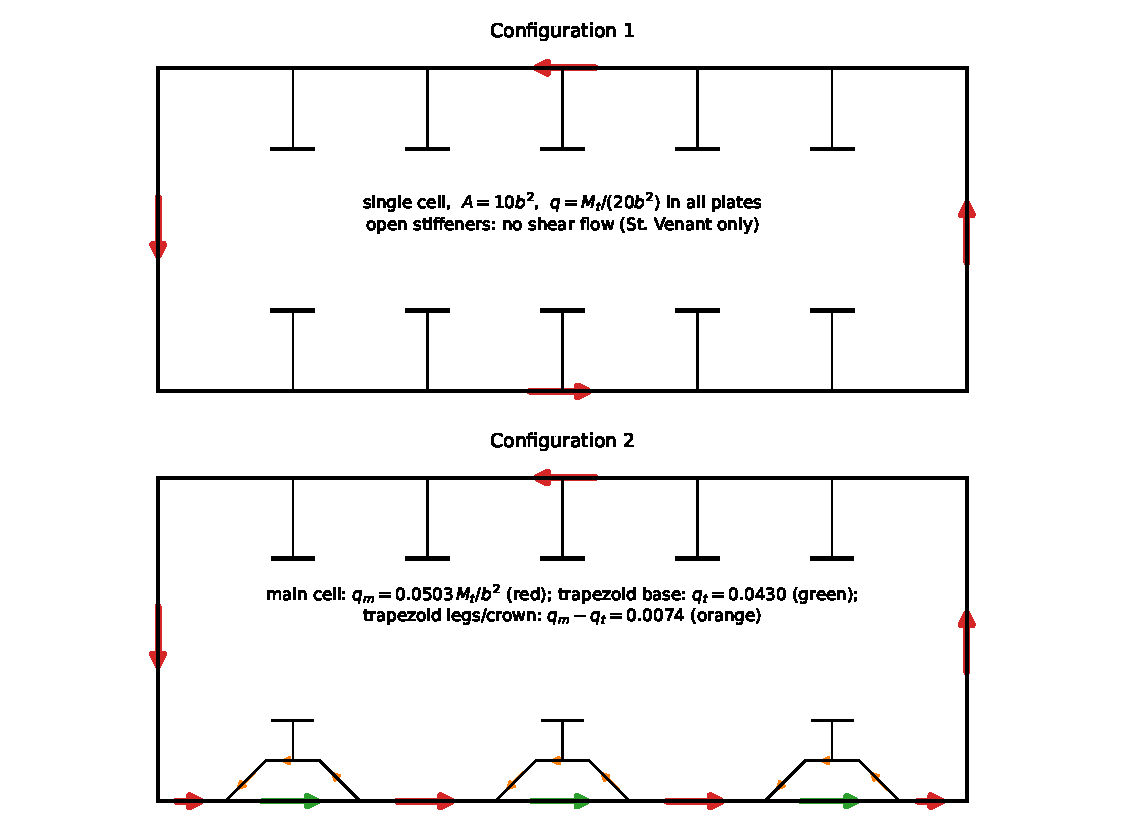
\includegraphics[width=0.95\textwidth]{figures/a3_flow}
  \caption{Shear flow (direction and relative magnitude) for configurations 1 and 2 under a CCW torsional moment; values from Question~3.3.}
  \label{fig:cfgflow}
\end{figure}

\section{T-stiffener versus L-stiffener}

Explain the consequences for the torsion stiffness contribution of open sections if a T-stiffener is exchanged for an L-stiffener, in case the web and flange dimensions remain the same. \textbf{(1 pt)}

\bigskip
The free (St.\,Venant) torsion constant of an open thin-walled profile is $I_p=\frac13\sum L_it_i^3$, i.e.\ it depends only on the lengths and thicknesses of the flat parts and not on how they are arranged. Moving the flange from the symmetric T position to the one-sided L position therefore leaves the contribution $\frac13\left(\tfrac{b}{2}t_p^3+\tfrac{b}{4}(2t_p)^3\right)=\tfrac56bt_p^3$ per stiffener unchanged. Only second-order effects differ: the junction correction (one free flange end instead of two, slightly different fillet term) and the position of the shear centre of the stiffener (at the web/flange junction in both cases, so the torque is applied identically). Consequences appear in \emph{warping} rather than in free torsion: the L-profile is asymmetric, has a (small) warping constant about its own shear centre and a larger tendency to lateral--torsional buckling (tripping) under compression, and its flange is loaded eccentrically. For the global torsion stiffness of the stiffened box these effects are negligible, and since the open contributions are anyway of order $(t_p/b)^2$ relative to the closed cell (Question~3.5), the exchange has no practical consequence for $I_p$.

\section{Shear flow components}

Calculate the shear flow components $q_i(b,t_p,M_t)$ for Configurations 1 and 2. \textbf{(4 pts)}

\bigskip
\emph{Configuration 1.} One cell with $A_1=5b\cdot2b=10b^2$ and $\oint\mathrm{d}s/t=14b/(2t_p)=7b/t_p$. Neglecting the torque carried by the open stiffeners (justified in Question~3.5; the exact fraction is $I_{p,open}/I_p\approx0.15(t_p/b)^2$):
\begin{equation}
  \boxed{\;q_1=\frac{M_t}{2A_1}=\frac{M_t}{20b^2}=0.0500\,\frac{M_t}{b^2}\;}\qquad
  I_{p,1,closed}=\frac{4A_1^2}{\oint\mathrm{d}s/t}=\frac{400b^4}{7b/t_p}=57.14\,b^3t_p .
\end{equation}

\emph{Configuration 2.} Two unknown flows: $q_m$ (main cell, $A_m=10b^2-3A_t=9.5625\,b^2$) and $q_t$ (each of the three identical trapezoid cells, $A_t=0.1458\,b^2$). Wall lengths over thickness (units $b/t_p$): box plating without the three trapezoid bases $(14-2.5)/2=5.75$; each trapezoid: legs $2\cdot0.3536/0.5=1.414$, crown $0.333/1=0.333$, base $0.833/2=0.417$. Cell equations \eqref{eq:bredt}:
\begin{align}
  \text{main:}\quad & \left[5.75+3(1.414+0.333)\right]q_m-3(1.414+0.333)\,q_t = 2\cdot9.5625\,b^2G\theta' \nonumber\\
  \text{trapezoid:}\quad & -(1.414+0.333)\,q_m+(1.414+0.333+0.417)\,q_t = 2\cdot0.1458\,b^2G\theta'
\end{align}
i.e.\ $10.99\,q_m-5.243\,q_t=19.125$, $-1.747\,q_m+2.164\,q_t=0.2917$ (per $bt_pG\theta'$), with solution $q_m=2.934$, $q_t=2.504$ ($\times bt_pG\theta'$). Then $I_{p,2,closed}=2A_mq_m+3\cdot2A_tq_t=(19.125\cdot2.934+0.875\cdot2.504)\,b^3t_p=58.30\,b^3t_p$, and per unit torque
\begin{equation}
  \boxed{\;q_m=0.0503\,\frac{M_t}{b^2},\qquad q_t=0.0430\,\frac{M_t}{b^2},\qquad q_m-q_t=0.0074\,\frac{M_t}{b^2}\ \text{(legs and crown)}\;}
\end{equation}
The trapezoid cells are so small that their flow is almost equal to that of the main cell, and the legs/crown carry only 15\% of $q_m$; the flow through the box plating ($0.0503$) is practically the single-cell value of configuration 1 ($0.0500$). Dimension check: $[q]=[M_t/b^2]=$N/m.

\section{Maximum shear stress}

\begin{enumerate}[label=\alph*.]
  \item Locate the position of maximum shear stress and obtain $\tau_{max,i}(b,t_p,M_t)$ for Configurations 1 and 2 (assuming $b\gg t_p$). \textbf{(3 pts)}

  With $b\gg t_p$ the stress in the open stiffeners, $\tau_{open}=G\theta't_{max}=2t_p\,M_t/I_p=0.035\,(t_p/b)\,M_t/(b^2t_p)$, is a factor $1.4\,t_p/b\ll1$ smaller than in the closed walls, and the closed walls carry the full torque. Configuration~1: uniform stress in all four box plates,
  \begin{equation}
    \boxed{\;\tau_{max,1}=\frac{q_1}{2t_p}=\frac{M_t}{40\,b^2t_p}=0.0250\,\frac{M_t}{b^2t_p}\;}\qquad(\text{everywhere in the box plating}).
  \end{equation}
  Configuration~2: box plating $\tau=0.0503/2=0.0252$; trapezoid base $0.0430/2=0.0215$; legs ($t_p/2$) $0.0074/0.5=0.0148$; crown $0.0074$. Hence
  \begin{equation}
    \boxed{\;\tau_{max,2}=0.0252\,\frac{M_t}{b^2t_p}\;}\qquad\text{in the box plating (sides, top and bottom plate between the trapezoids)}.
  \end{equation}

  \item Compare the outcomes of configuration 1 and 2 to the (given) outcome of configuration 3 and discuss the differences. \textbf{(2 pts)}

  Configuration 3: $\tau_{max,3}=0.02769\,M_t/(b^2t_p)$, i.e.\ 11\% higher than configurations 1 ($0.0250$) and 2 ($0.0252$), which are practically equal. In configurations 1 and 2 the torque is carried by one large cell with a nearly uniform shear flow $M_t/(2A)$ in $2t_p$ plating. In configuration 3 the webs divide the box into four cells in series across the breadth and the six trapezoids into small cells; the cell flows differ (larger in the two central cells than in the outer cells), so that the plating between the central trapezoids carries a higher net flow ($0.054\,M_t/b^2$ in the own model) than the average $0.05\,M_t/b^2$. The subdivision thus concentrates shear flow in the middle of the top and bottom plates and raises the peak stress, while the total enclosed area (and therefore the average flow) is unchanged. In the own model of configuration 3 the thin legs ($t_p/2$) of the outer trapezoids come close to the plating stress ($0.025$), which shows that thin walls of small cells adjacent to large cells are potential hot spots.
\end{enumerate}

\section{Specific torsion stiffness and strength}

\begin{enumerate}[label=\alph*.]
  \item Calculate the (specific) torsion stiffness $I_{p,i}(b,t_p)$ and strength $M_{t,i}(b,t_p,\tau_{max})$ for Configurations 1 and 2. \textbf{(3 pts)}

  Closed parts from Question~3.3; open parts $\frac13\sum Lt^3$: configuration 1 has ten T's of $\frac13(\tfrac b2t_p^3+\tfrac b4\cdot8t_p^3)=\tfrac56bt_p^3$, configuration 2 five large T's and three small T's of $\frac13(\tfrac b4+\tfrac b4)t_p^3=\tfrac16bt_p^3$:
  \begin{align}
    I_{p,1}&=57.14\,b^3t_p+8.33\,bt_p^3=57.14\,b^3t_p\left[1+0.146\,(t_p/b)^2\right]\approx\boxed{57.1\,b^3t_p}\\
    I_{p,2}&=58.30\,b^3t_p+4.67\,bt_p^3=58.30\,b^3t_p\left[1+0.080\,(t_p/b)^2\right]\approx\boxed{58.3\,b^3t_p}
  \end{align}
  Strength (torque at which $\tau_{max}$ is reached in the governing wall, Question~3.4a):
  \begin{equation}
    M_{t,1}=\frac{b^2t_p\tau_{max}}{0.0250}=\boxed{40.0\,b^2t_p\tau_{max}},\qquad
    M_{t,2}=\frac{b^2t_p\tau_{max}}{0.02516}=\boxed{39.7\,b^2t_p\tau_{max}} .
  \end{equation}
  Order-of-magnitude check: $M_{t,1}=2A\,t\,\tau_{max}=2\cdot10b^2\cdot2t_p\tau_{max}=40\,b^2t_p\tau_{max}$ (Bredt's first formula), and $I_{p,1}=4A^2t/\oint\mathrm{d}s$ (Bredt's second formula).

  \item Compare the outcomes of Configurations 1 and 2 to the (given) outcome of Configuration 3 and discuss the origin of possible differences. \textbf{(2 pts)}

  \begin{center}\small
  \begin{tabular}{lccc}
    \toprule
     & config.\ 1 & config.\ 2 & config.\ 3 (given) \\
    \midrule
    $I_p$ [$b^3t_p$] & 57.1 & 58.3 & 61.6 \\
    $\tau_{max}$ [$M_t/(b^2t_p)$] & 0.0250 & 0.0252 & 0.0277 \\
    $M_t$ [$b^2t_p\tau_{max}$] & 40.0 & 39.7 & 36.1 \\
    \bottomrule
  \end{tabular}
  \end{center}
  \emph{Stiffness.} Configuration 3 is 8\% stiffer than 1 and 6\% stiffer than 2. All three configurations enclose the same total area $10b^2$ with the same $2t_p$ plating, so the single-cell value $57.1\,b^3t_p$ is the base value. Adding closed walls inside a closed section never reduces $I_p$: the webs, legs and crowns of configuration 3 provide additional parallel shear paths, the cell flows redistribute (larger flows in the central cells) and the effective $\oint\mathrm{d}s/t$ seen by the flow decreases, which yields the 8\% gain. In configuration 2 only the three small bottom trapezoids are closed, which gives 2\%; its open T-stiffeners, like all stiffeners of configuration 1, contribute only $\mathcal O\big((t_p/b)^2\big)$. \emph{Strength.} Configuration 3 is the weakest (10\% lower than 1) because the subdivision into cells with unequal flows produces a local peak in the plating between the central trapezoids (Question~3.4b), whereas the single-cell configurations load their plating uniformly. Thus, for the same plating, converting open stiffeners into closed cells increases the stiffness noticeably, but may reduce the torsional strength when the cell arrangement produces uneven shear flows; the amount of stiffener material also differs between the configurations, so the comparison is not at equal weight.

  \item For Configurations 1 and 2 split the relative stiffness and strength contributions for the open and closed parts and discuss the differences. \textbf{(2 pts)}

  At the common twist rate $\theta'$ the torque splits in proportion to the torsion constants, $M_{closed}:M_{open}=I_{p,closed}:I_{p,open}$:
  \begin{center}\small
  \begin{tabular}{lcc}
    \toprule
     & config.\ 1 & config.\ 2 \\
    \midrule
    $I_{p,closed}$ & $57.14\,b^3t_p$ & $58.30\,b^3t_p$ \\
    $I_{p,open}$ & $8.33\,bt_p^3$ & $4.67\,bt_p^3$ \\
    $I_{p,open}/I_{p,closed}$ & $0.146\,(t_p/b)^2$ & $0.080\,(t_p/b)^2$ \\
    e.g.\ $b/t_p=50$ & $5.8\times10^{-5}$ & $3.2\times10^{-5}$ \\
    $\tau_{open,max}/\tau_{closed,max}$ & $1.40\,t_p/b$ & $1.36\,t_p/b$ \\
    \bottomrule
  \end{tabular}
  \end{center}
  The open stiffeners carry a fraction $\mathcal O\big((t_p/b)^2\big)$ of the torque, i.e.\ well below $10^{-3}$ for any realistic plate slenderness, and their contribution to the stiffness is negligible. For strength the open parts are irrelevant as well: their maximum stress is $G\theta't_{max}$, a factor $\approx1.4\,t_p/b$ (a few per cent) below the stress in the closed walls, so the closed cells govern both stiffness and strength. In configuration 2 the ``open'' share is smaller than in configuration 1 because three of the bottom stiffeners have become closed trapezoids and the small T's have thinner flanges; the closed share is correspondingly 2\% larger. The practical conclusion is that open stiffeners are provided for local plate bending and buckling, not for torsion, and that torsional stiffness must come from closed cells (hatch covers, wing tanks, double bottom, torsion boxes).
\end{enumerate}


\part{Part 2}
\chapter{Idealised Section U --- Analytical vs.\ ANSYS}
\label{ch:assignment4}

\begingroup\itshape Assignment 4 --- 20 points\endgroup

\bigskip
Revisit idealised section BU without a hatch cover. Consider the U-shaped structure of Assignment~2.5--2.6 with breadth $A = 8a$, depth $B = 5a$, bottom thickness $t_{bp} = 6.5\,t_p$, and side-shell thickness $t_{sp} = 3.5\,t_p$.

\section{Analytical model vs.\ ANSYS model}

For section B, use the idealised U-shaped model (i.e., without decks and stringers) to answer the following questions. Match the parameters of the analytical model to the parameters found in the ANSYS script. Note the controls for warping constraints; the different plots can be extracted using General Postproc.

\subsection{Free warping shear stress}

Calculate and compare the analytical and numerical free warping shear stress components $\tau_{xy}$ and $\tau_{xz}$ through-thickness distribution in all structural members. Use $I_p$ obtained in Assignment~2.6. \textbf{(5 pts)}

\begin{enumerate}[label=\roman*.]
  \item Calculate the analytical free warping shear stress components $\tau_{xy}(y,z)$ and $\tau_{xz}(y,z)$ in all structural members. \textbf{(1 pt)}

  \textit{Answer.}

  \item Present a plot (screen capture from the UI) of the numerical (ANSYS) free warping shear stress components $\tau_{xy}$ and $\tau_{xz}$ in all structural members. Explicitly state which input and settings (mesh size, convergence, element type, etc.) you used in ANSYS and why. \textbf{(1 pt)}

  \textit{Answer.}

  \item Present both the analytical and numerical solution in a single plot per shear stress component for comparison. \textbf{(1 pt)}

  \textit{Answer.}

  \item Discuss (the differences in) the through-thickness distribution and maximum values between the analytical and numerical method. \textbf{(2 pts)}

  \textit{Answer.}
\end{enumerate}

\subsection{Free warping displacement}

Calculate and compare the analytical and numerical free warping displacement distribution $u(s)$. Use $\omega(s)$ obtained in Assignment~2.5. \textbf{(5 pts)}

\begin{enumerate}[label=\roman*.]
  \item Calculate the analytical free warping displacement distribution $u(s)$. \textbf{(1 pt)}

  \textit{Answer.}

  \item Present a plot of the numerical (ANSYS) free warping displacement distribution $u(s)$ in all structural members. Explicitly state which input and settings you used in ANSYS and why. \textbf{(1 pt)}

  \textit{Answer.}

  \item Present both the analytical and numerical solution in a single plot for comparison. \textbf{(1 pt)}

  \textit{Answer.}

  \item Discuss (the differences in) the $s$ distribution (i.e., the distribution over the sectorial coordinate $s$) and extreme values between the analytical and numerical method. \textbf{(2 pts)}

  \textit{Answer.}
\end{enumerate}

\subsection{Constrained warping stress}

Calculate and compare the analytical and numerical constrained warping stress distribution $\sigma_{xx}(s)$. Use $I_w$ obtained in Assignment~2.6. \textbf{(5 pts)}

\begin{enumerate}[label=\roman*.]
  \item Calculate the analytical constrained warping stress distribution $\sigma_{xx}(s)$. \textbf{(1 pt)}

  \textit{Answer.}

  \item Present a plot of the numerical (ANSYS) constrained warping stress distribution $\sigma_{xx}(s)$ in all structural members. Explicitly state which input and settings you used in ANSYS and why. \textbf{(1 pt)}

  \textit{Answer.}

  \item Present both the analytical and numerical solution in a single plot for comparison. \textbf{(1 pt)}

  \textit{Answer.}

  \item Discuss (the differences in) the $s$ distribution and extreme values between the analytical and numerical method. \textbf{(2 pts)}

  \textit{Answer.}
\end{enumerate}

\subsection{Constrained warping shear stress}

Calculate and compare the constrained warping shear stress distribution $\tau_{xy}(s)$ and $\tau_{xz}(s)$. Use $S_\omega(s)$ obtained in Assignment~2.5. \textbf{(5 pts)}

\begin{enumerate}[label=\roman*.]
  \item Calculate the analytical distributions of the constrained warping shear stress components $\tau_{xy}(s)$ and $\tau_{xz}(s)$. \textbf{(1 pt)}

  \textit{Answer.}

  \item Present a plot of the numerical (ANSYS) constrained warping shear stress components $\tau_{xy}$ and $\tau_{xz}$ in all structural members. Explicitly state which input and settings you used in ANSYS and why. \textbf{(1 pt)}

  \textit{Answer.}

  \item Present both the analytical and numerical solution in a single plot per shear stress component for comparison. \textbf{(1 pt)}

  \textit{Answer.}

  \item Discuss (the differences in) the through-thickness and $s$ distribution and maximum values between the analytical and numerical method. \textbf{(2 pts)}

  \textit{Answer.}
\end{enumerate}

\chapter{Combined Torsional Analysis}
\label{ch:assignment5}

\begingroup\itshape Assignment 5 --- 17 points\endgroup

\bigskip
For the generalised torsion equation use the parameters listed in Table~\ref{tab:torsion-constants}. Each section of the vessel has a length of 20~m. The vessel is subject to a uniform torsional load of 100~MNm. Use a Young's modulus of 205~GPa and a shear modulus of 79~GPa.

\begin{table}[h]
  \centering
  \caption{Torsion and warping constants for vessel sections.}
  \label{tab:torsion-constants}
  \begin{tabular}{lcccccc}
    \toprule
     & A & B1 & B2 & BU & BUH & C \\
    \midrule
    $I_p$ [m$^4$] & 6.72 & 1.05 & 0.86 & $8.71\times10^{-4}$ & 7.83 & 6.05 \\
    $I_w$ [m$^6$] & 4.45 & 23.6 & 25.7 & 22.6 & 2.71 & 4.00 \\
    \bottomrule
  \end{tabular}
\end{table}

\section{Generalised torsion equation and boundary conditions}

Provide the generalized torsion equation and the necessary boundary conditions (both between adjacent sections and at the ends of the vessel) to solve it for the entire ship (composed of five sections). Explain the choice of boundary conditions.
\begin{quote}
\emph{Hint: assume zero twist rate at the intersections of the sections due to the bulkheads with large torsional stiffness.}
\end{quote}
\textbf{(5 pts)}

\bigskip
\textit{Answer.}

\section{Twist deformation and rate over the ship length}

Use the torsional characteristics of each of the 5 ship sections to calculate and plot the twist deformation and rate over the ship length under constant torsional moment for the situation with configuration B1 and B2 (many and few cells).
\begin{quote}
\emph{See the example file on Brightspace on how to obtain the solution of the general torsion equation using Maple.}
\end{quote}
\textbf{(7 pts)}

\bigskip
\textit{Answer.}

\section{Open versus closed hatch covers}

Compare the results of a vessel subject to constant torsional moment with all 3 hatch covers closed (BUH) and all open (BU) for configuration B. \textbf{(5 pts)}

\begin{enumerate}[label=\alph*.]
  \item Compare the plot of the rotation over the length, and discuss differences. \textbf{(2 pts)}

  \textit{Answer.}

  \item Compare the plot of the twist rate over the length, and discuss differences. \textbf{(2 pts)}

  \textit{Answer.}

  \item Compare the improvement with respect to the maximum twist rate. \textbf{(1 pt)}

  \textit{Answer.}
\end{enumerate}

\chapter{Scientific Literature}
\label{ch:assignment6}

\begingroup\itshape Assignment 6 --- 7 points\endgroup

\bigskip
Carefully read \textcite{SilvaCampillo2022} (Brightspace~$>$~Readings~$>$~Other references), and answer the following questions.

\section{Adapting the torsion box for a heavier storm}

Given the conclusions drawn by the authors, how would you adapt the dimensions of the torsion box for a container ship that has a heavier 10-year return period storm and why? (max.\ 100 words, no calculations needed) \textbf{(3 pts)}

\bigskip
\textit{Answer.}

\section{Role of plate thickness}

Why do the authors not vary plate thicknesses in the torsion box? What is the role of plate thickness in the structural response to torsion? (100 words) \textbf{(4 pts)}

\bigskip
\textit{Answer.}

\chapter{Structural Monitoring}
\label{ch:assignment7}

\begingroup\itshape Assignment 7 --- 8 points\endgroup

\section{Inclinometer array for warping identification}

Conventional inclinometers are rotation sensors used to measure the pitching and rolling of a vessel. High-end electronic inclinometers can provide resolutions in the order of microradians, hence may also be used to measure the twist angle at any point along the ship. If an array of inclinometers is used as a monitoring system, how can the contributions of free and constrained warping be identified with the help of the generalised torsion equation (inertia effects are neglected)? Furthermore, how can the location of the maximum warping stress be identified? \textbf{(4 pts)}

\bigskip
An array of $n$ inclinometers mounted along the length (e.g.\ on the centre line at every bulkhead and at mid-hold) measures the roll angle $\theta_k(t)$ at stations $x_k$. Subtracting the rigid-body roll (the common part, e.g.\ the value at a reference station or the mean) leaves the elastic twist $\theta(x_k)-\theta(x_{ref})$ along the ship. Fitting a smooth function (piecewise polynomial or the closed-form solution \eqref{eq:gensol} with $C_{1i},C_{2i}$ as unknowns per section) to these samples gives $\theta(x)$ and, by differentiation, the twist rate $\theta'(x)$, the curvature $\theta''(x)$ and $\theta'''(x)$. The generalised torsion equation \eqref{eq:gte} then separates the two load paths directly:
\begin{equation}
  M_t(x)=\underbrace{GI_p\,\theta'(x)}_{\text{free (St.\,Venant) warping}}\;\underbrace{-\,EI_w\,\theta'''(x)}_{\text{constrained warping torque } M_\omega},\qquad
  B_\omega(x)=-EI_w\,\theta''(x)\ \ \text{(bimoment)}.
\end{equation}
With the known section properties ($I_p$, $I_w$ from the drawings, as in Table~\ref{tab:torsion-constants}) the measured $\theta'$ gives the St.\,Venant part and the measured $\theta'''$ the warping part; where $\theta'$ is constant (linear $\theta$, $\theta''=\theta'''=0$) warping is free and the whole torque is St.\,Venant, whereas a $\theta'$ that decreases towards a bulkhead ($\theta''\ne0$) reveals the constrained-warping contribution, in the form of the boundary layers of Figure~\ref{fig:a5BUBUH}. In practice $\theta'''$ from three numerical differentiations is noisy, so the inclinometer data should be fitted with the analytical solution per section (which has only the constants $C_{1i}$, $C_{2i}$ and the unknown $M_t$) rather than differentiated numerically; the fit also identifies the actual torque $M_t(x)$ and, from the size of the boundary layers, the effective restraint provided by the bulkheads. Because inertia effects are neglected, the quasi-static equation can be applied at every time instant.

The warping normal stress is $\sigma_{xx}(s,x)=-E\,\omega(s)\,\theta''(x)$. Its maximum over the length therefore lies where $|\theta''|$ -- the curvature of the twist, i.e.\ the slope of the measured $\theta'(x)$ -- is largest, and over the section at the point of largest $|\omega|$ (the hatch coaming / top of the side shell for an open section, $\omega=\pm13.3a^2$ in Assignment~2.5). From the fitted $\theta'(x)$ the positions of maximum $|\theta''|$ are found: for the constrained holds these are the sections adjacent to the transverse bulkheads (and the engine-room front bulkhead), where $\theta'$ changes fastest; in the middle of a hold $\theta''=0$ and the warping stress vanishes. Thus the inclinometer array locates the hot spots without strain measurements, and the bimoment $B_\omega=-EI_w\theta''$ there gives the stress level $\sigma_{xx,max}=B_\omega\omega_{max}/I_w$, which can be checked against the values predicted in Assignment~5 (e.g.\ $|\theta''|_{max}=1.6\times10^{-4}$~m$^{-2}$ next to the bulkheads for B1).

\bigskip
\noindent\textbf{Final answer.} Fit the elastic twist $\theta(x)$ from the inclinometer array with the generalised torsion solution; $GI_p\theta'$ is the free-warping (St.\,Venant) torque and $-EI_w\theta'''$ the constrained-warping torque. The maximum warping stress occurs where $|\theta''|$ is largest -- at the sections next to the (bulkhead) warping restraints -- and at the point of maximum $|\omega|$ in that section.

\section{Long-base strain gauges}

Consider a cross-section instrumented for longitudinal normal strain monitoring on the inner shell (Figure~12 of the brief). The total strain is the combination of the horizontal bending, vertical bending and warping strain, $\varepsilon_{xx,tot}=\varepsilon_{xx,vb}+\varepsilon_{xx,hb}+\varepsilon_{xx,warp}$. In fatigue assessment, a multiaxial stress state may significantly reduce the lifetime of a structure. Through a monitoring system composed of long-base strain gauges, the longitudinal normal strain at any point along the inner shell of a cross section can be measured. Discuss how the torsion and vertical and horizontal bending responses may be separated using multiple long-base strain gauges in the cross-section. Should these strain gauges be placed on a cross-section close to a bulkhead or away from it? \textbf{(4 pts)}

\bigskip
At a point $(y_k,z_k)$ of the section with sectorial coordinate $\omega_k$ (pole at the shear centre, principal sectorial origin), beam theory gives
\begin{equation}
  \varepsilon_{xx}(y_k,z_k)=\frac{N}{EA}+\frac{M_y}{EI_{yy}}\,z_k-\frac{M_z}{EI_{zz}}\,y_k+\frac{B_\omega}{EI_w}\,\omega_k ,
  \label{eq:strainsep}
\end{equation}
where $z$ is measured from the neutral axis of vertical bending, $y$ from the centre line, and the axial force $N$ is included for generality (it is zero for pure hull-girder loading but not necessarily for temperature effects). Each gauge $k$ yields one linear equation in the unknown generalised loads $(N,M_y,M_z,B_\omega)$, with known coefficients $(1/A,\ z_k/I_{yy},\ -y_k/I_{zz},\ \omega_k/I_w)$ from the section geometry. With at least four gauges at suitably chosen positions (more for a least-squares fit) the system is solved at every time step and the three responses are separated. The choice of positions exploits the symmetries of the U-shaped section (Figure~12): vertical bending strain is \emph{symmetric} in $y$ and varies linearly with $z$; horizontal bending strain is \emph{antisymmetric} in $y$ and independent of $z$; warping strain is \emph{antisymmetric} in $y$ (like $\omega$ in Figure~\ref{fig:omega}) but varies linearly with $z$ along the sides and changes sign at $z=e$, and is also antisymmetric along the bottom. A practical arrangement on the red surfaces of Figure~12 is a pair of gauges high on the port and starboard inner side shells ($\pm y_s$, $z_1$) and a pair low on the sides or at the bottom corners ($\pm y_s$, $z_2$):
\begin{itemize}
  \item sum of a port/starboard pair: $\varepsilon_P+\varepsilon_S=2\left(N/EA+M_yz/EI_{yy}\right)$ -- the antisymmetric (horizontal bending and warping) parts cancel; two such sums at $z_1\ne z_2$ give $M_y$ (and $N$);
  \item difference of a pair: $\varepsilon_P-\varepsilon_S=2\left(-M_zy_s/EI_{zz}+B_\omega\omega(z)/EI_w\right)$ -- the symmetric parts cancel; since $\omega$ varies with $z$ and $y_s$ does not, the differences at two heights $z_1$, $z_2$ separate $M_z$ from $B_\omega$ (the warping part changes sign across $z=e$, the horizontal bending part does not); a gauge near $z=e$, where $\omega\approx0$, measures horizontal bending without warping contamination, and a gauge at the top of the side, where $|\omega|$ is largest, is the most sensitive to warping.
\end{itemize}
The separation requires that the section is instrumented at one $x$-position with all gauges (same $M_y$, $M_z$, $B_\omega$), that local effects (plate bending between stiffeners, hatch-corner concentrations) are averaged out -- which is exactly what long-base gauges do -- and that $\omega_k$, $I_w$ etc.\ are known from the structural drawings. Combining the strain-derived $B_\omega(x)$ with the inclinometer-derived $\theta''(x)$ of Question~7.1 provides a consistency check ($B_\omega=-EI_w\theta''$).

\emph{Close to or away from a bulkhead?} The warping strain is proportional to the bimoment, which is largest next to a warping restraint and zero at mid-hold (Assignment~5): a section close to a bulkhead therefore gives the largest, well-conditioned warping signal and coincides with the fatigue-critical location (maximum $\sigma_{xx,warp}$ superimposed on the bending stresses -- the multiaxial state the question refers to). Directly at the bulkhead, however, the strain field is disturbed by the local stiffness of the bulkhead, its brackets and the hatch-end coaming (three-dimensional stress state, shear lag), and beam theory \eqref{eq:strainsep} is not valid. The recommended position is therefore \emph{close to the bulkhead but outside its local influence zone} -- of the order of half the section depth to one depth away (a few metres), i.e.\ well within the boundary layer $1/\lambda$ for an open hold (which extends over the full hold for BU) but away from the local details. Bending moments vary slowly along the hold, so they are not affected by this choice. For a complete picture of the fatigue loading a second, mid-hold section (where warping is nearly zero) is useful to isolate the bending responses and to calibrate the warping identification.

\bigskip
\noindent\textbf{Final answer.} Use $\ge4$ long-base gauges in one section at symmetric port/starboard positions and two heights; sums of pairs isolate vertical bending (and axial force), differences at two heights separate horizontal bending from warping via the known $\omega(s)$ and $I_w$ (least-squares solution of \eqref{eq:strainsep}). Place the instrumented section close to a bulkhead (largest bimoment, fatigue-critical) but outside the local disturbance zone of the bulkhead, with a mid-hold section as bending reference.


% Use letters for the chapter numbers of the appendices.
\appendix

\chapter{Maple and ANSYS Files}
\label{ch:appendix}

This appendix collects the supporting Maple worksheets and ANSYS input files used to obtain the analytical and numerical results presented in the main report (e.g., the example Maple files referenced in Assignments~3.3 and~5.2, and the ANSYS models used throughout Assignment~4).

\section{Maple worksheets}

\textit{Include (excerpts of) the Maple worksheets used for the analytical derivations here, e.g.\ as a \texttt{verbatim} listing or exported code.}

\section{ANSYS input files}

\textit{Include the ANSYS input/settings (mesh, element type, boundary conditions, load application) used for the numerical models here.}


% Chapters without numbers in the back
\backmatter%
\printbibliography[heading=bibintoc]

\MakeCoverBack%

\end{document}

